\subsection{Approximation of a porous medium} \label{sec:approx-porous-medium}

	\begin{figure}[H]
		\centering
		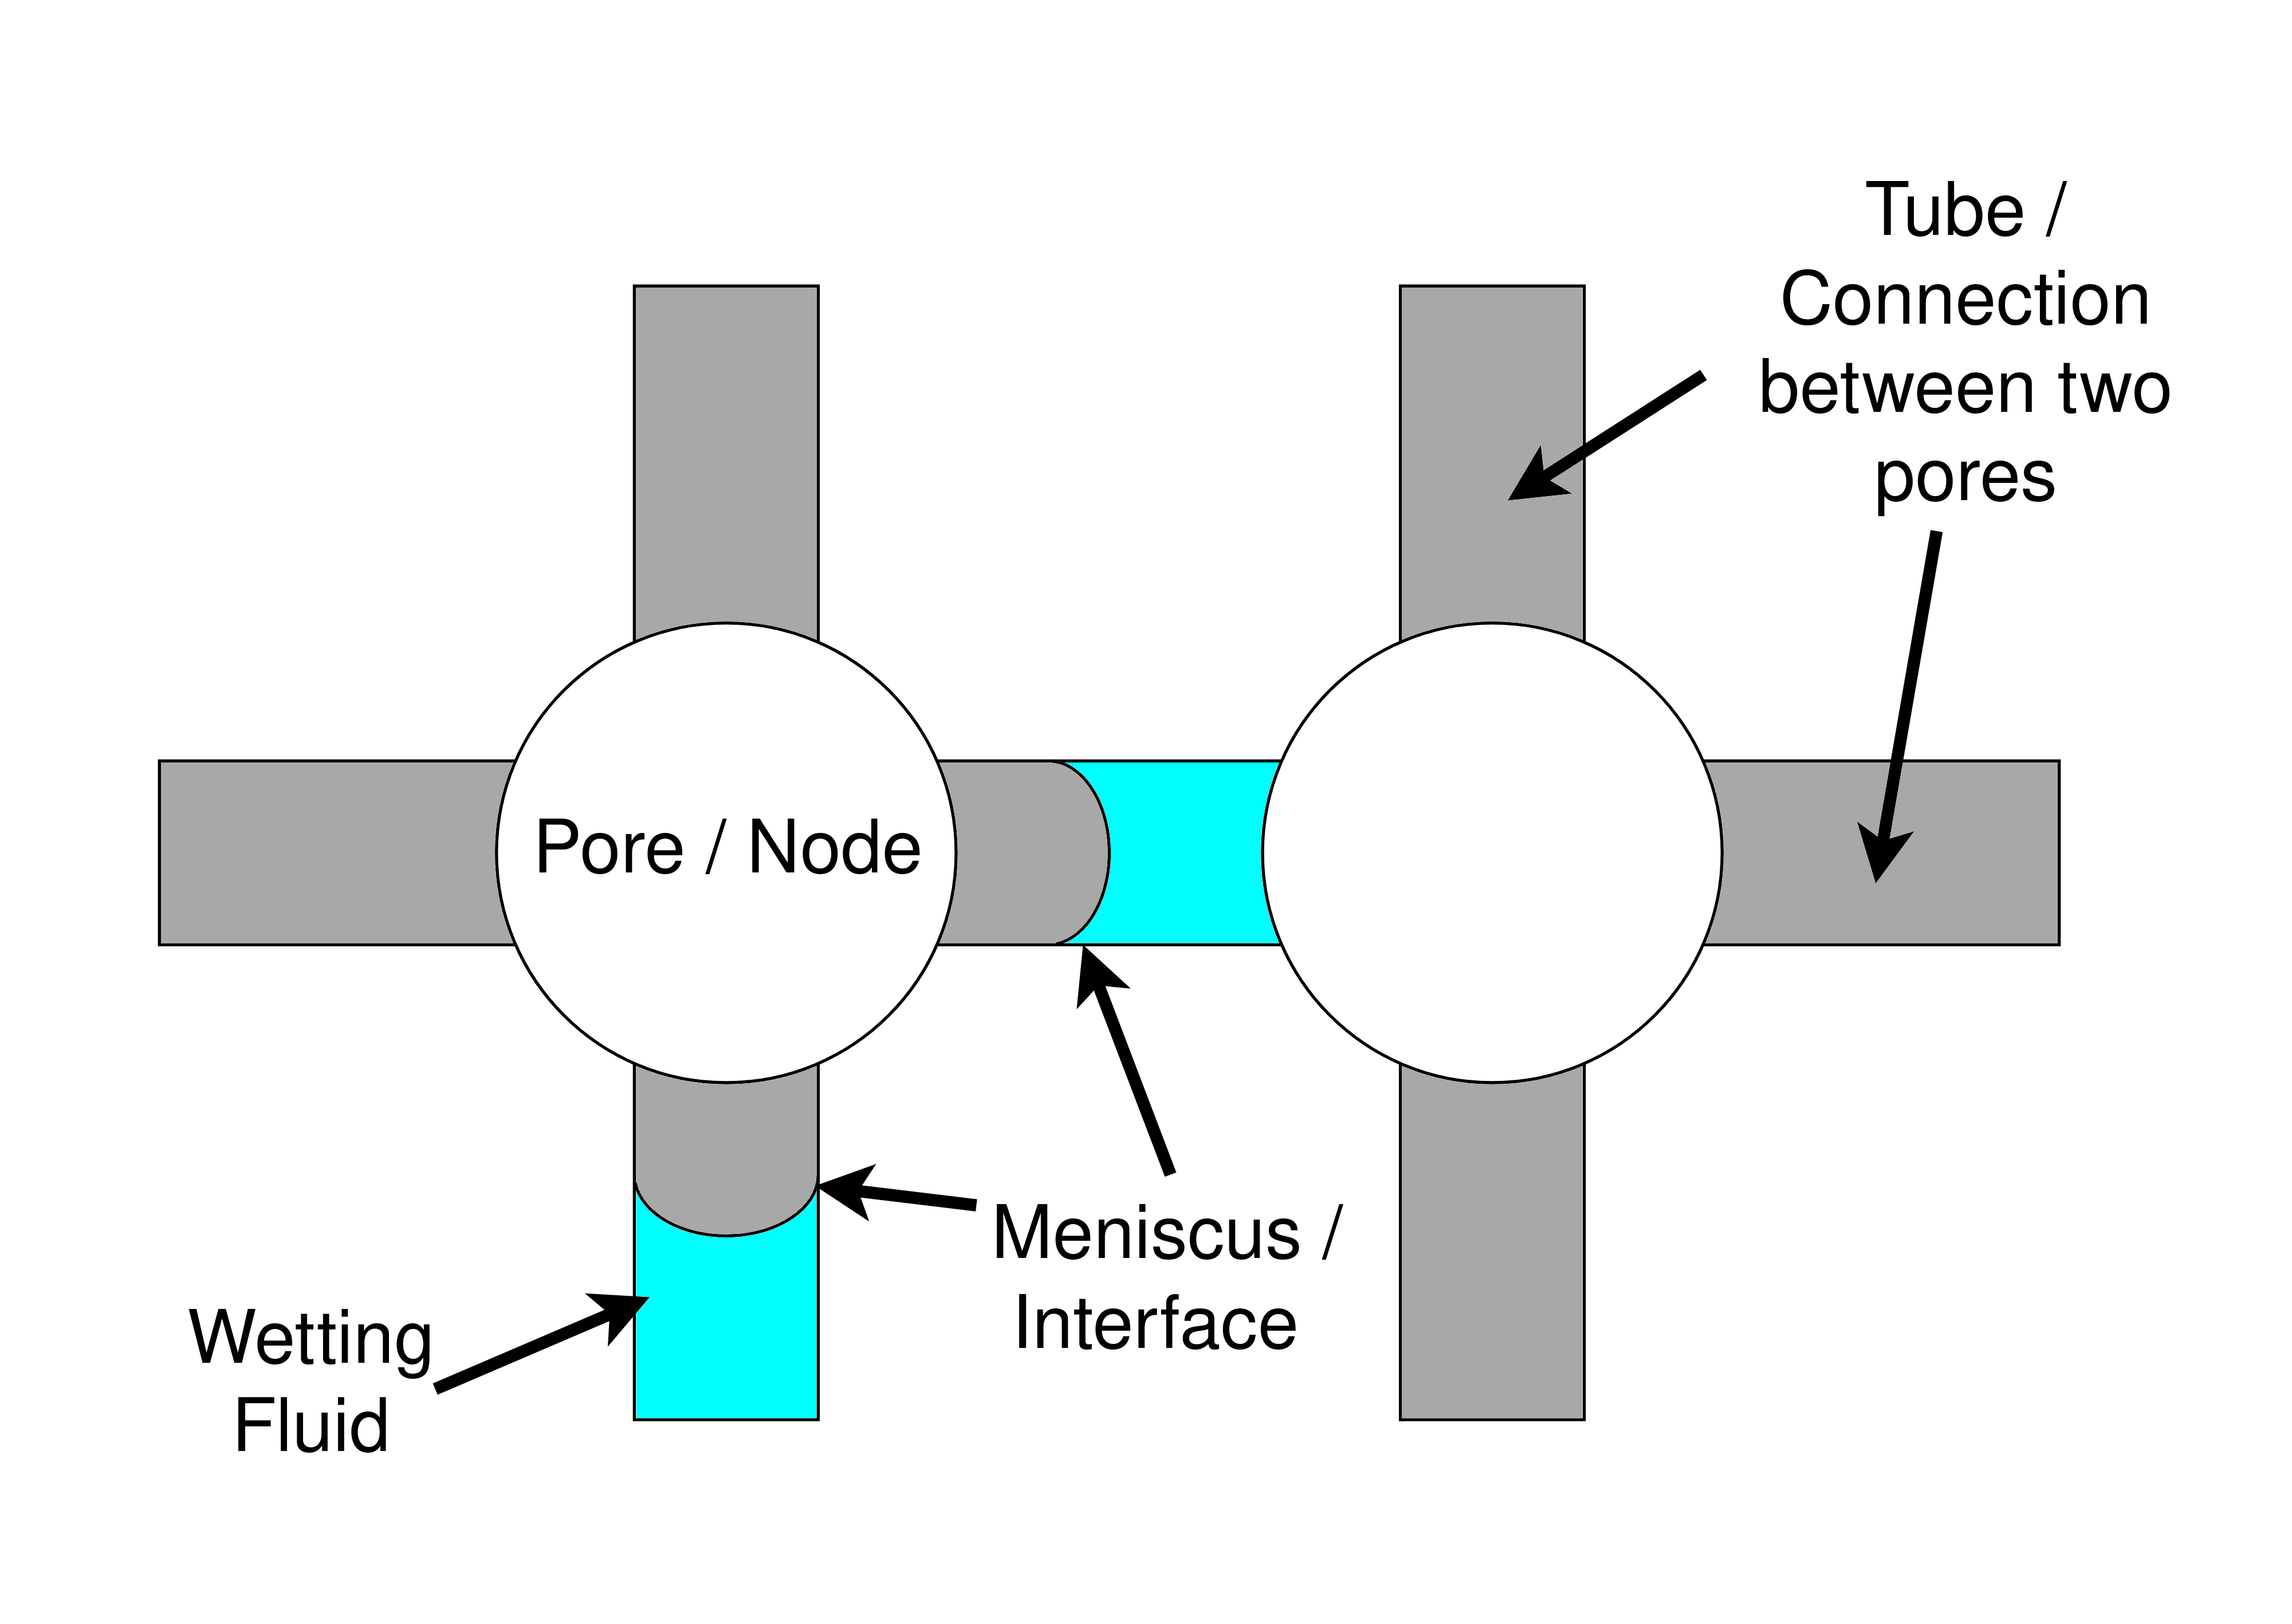
\includegraphics[height=7cm]{fig_descp-of-model}
		\caption{Capillary and pore as tube and node}
		\label{fig:descp-of-model}
	\end{figure}
	
	A porous medium consists of pores, which are connected by capillaries. The pores are represented by nodes, while the capillaries are represented by tubes, as shown in figure \ref{fig:descp-of-model}.
	
	Denotations for our model:
	
	\begin{itemize}
		\item Our model is two-dimensional 
		\item Each node is connected to 4 other nodes through tubes, shown in figure \ref{fig:simple-5-nodes}. They may be connected to less than 4 nodes, when they are located on the boundaries.
		\item The color cyan denotes wetting fluid, while the color gray denotes non-wetting fluid.
	\end{itemize}
	
	Assumptions model:
	
	\begin{itemize}
		\item The fluids are not compressible.
		\item The volume of the node is not taken into consideration and is assumed to be zero.
		\item All tubes are of equal length and cylindrical. The tubes can have different radii.
		\item The capillary pressure is zero inside the node.
		\item A tube can have a maximum of 2 menisci.
		\item During flow, when both cyan and gray fluid enters one node, then the fluids are distributed such that the cyan fluid is distributed first to the thinner tubes.
		\item During flow, if a tube has more than two meniscus, then there are combined together such that the center of mass of each fluid remains the same.
	\end{itemize}
	
	Note that the assumption of zero volume of node would not change the mixing of different fluids. Let us assume that a node with non-zero volume is filled with gray fluid is invaded by cyan fluid. Since the cyan fluid is distributed first, it immediately reaches the ends of the other tubes connected to the node. The assumption of zero volume of node only affects how the saturation is calculated, never the less it was assumed to be zero to keep the calculations for the flow simple.

\subsection{Set of linear equations for a node} \label{sec:linear-equ}
	\begin{figure}[H]
		\centering
		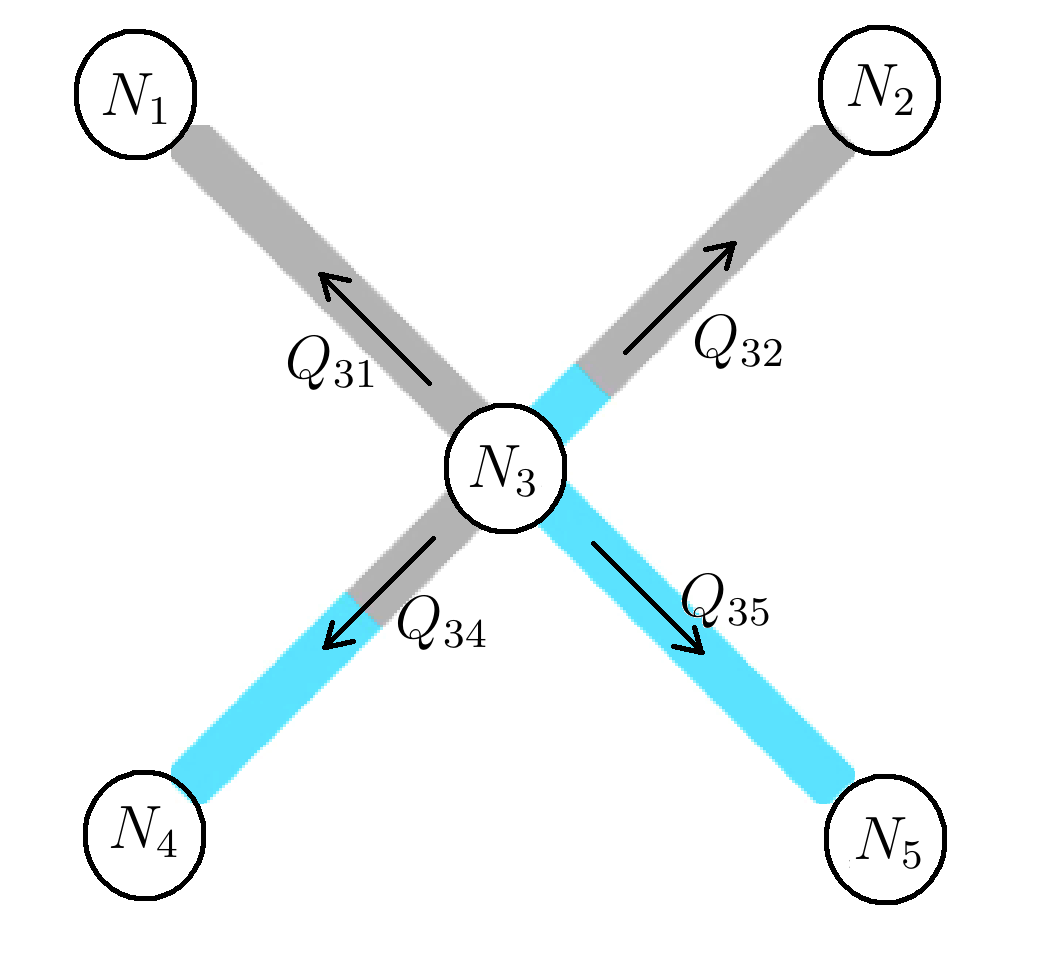
\includegraphics[height=8cm]{fig_simple-5-nodes}
		\caption{Denotation of flow rates in tubes for one node connected to 5 other nodes}
		\label{fig:simple-5-nodes}
	\end{figure}
	
	Let the flow rate in a tube be given by,
	\begin{equation}  \label{eq:flow-rate-simple-coeff}
		Q_{ij} = A_{ij}\Delta P_{ij} + B_{ij}
	\end{equation}
	
	Here, $Q_{ij}$ is the flow rate form node $N_i$ to node $N_i$. $A_{ij}$ and $B_{ij}$ are real constants. Here $\Delta P_{ij} = P_i - P_j$, where $N_i$ is kept at a pressure of $P_i$ and $N_j$ at a pressure of $P_j$. The detailed form is given by equation \ref{eq:main-flow-rate-with-s}
	
	During simulation, we produce a set of linear equations. We iterate through each node, write equations of flow rates for each tube connected to the node, and equate the sum to zero. For each node, we get one linear equation. For figure\ref{fig:simple-5-nodes}:
	
	\begin{equation}
		Q_{3j} = A_{3j}\Delta P_{3j} + B_{3j}
	\end{equation}

	Due to the conservation of volume, we have:
	\begin{equation}
		\sum_{k} Q_{3k} = 0
	\end{equation}
	
	Where $k = {1, 2, 4, 5}$.
	
	Note that all $Q$'s point outward. The $Q$'s will have different signs in order to preserve the law of conservation of volume. 
	
	For fluid flowing out of $N_3$,
	\begin{equation}
		Q_{3j} > 0
	\end{equation}
	
	For fluid flowing into $N_3$,
	\begin{equation}
		Q_{3j} < 0
	\end{equation}
	
	Let us assume that the pressures at all nodes are known, except $N_3$. Then, the set of linear equations is:
	
	\begin{equation}
		\begin{pmatrix}
			1 & 0 & 0 & 0 & 0 & P_{1}\\
			0 & 1 & 0 & 0 & 0 & P_{2}\\
			-A_{31} & -A_{32} & (A_{31} + ... + A_{35}) & -A_{34} & -A_{35} & -(B_{31} + ... + B_{35})\\
			0 & 0 & 0 & 1 & 0 & P_{4}\\
			0 & 0 & 0 & 0 & 1 & P_{5}
		\end{pmatrix}
	\end{equation}
	
\subsection{Multi-phase flow in a node} \label{sec:multi-phase-flow}
	The novelty of our model is how we distribute phases in the nodes. When more than one phase flows into a node, the wetting fluid first enters the tube with the thinner radius. This is to minimize the energy of the system. Below is an example:
	
	\begin{figure}[H]
		\centering
		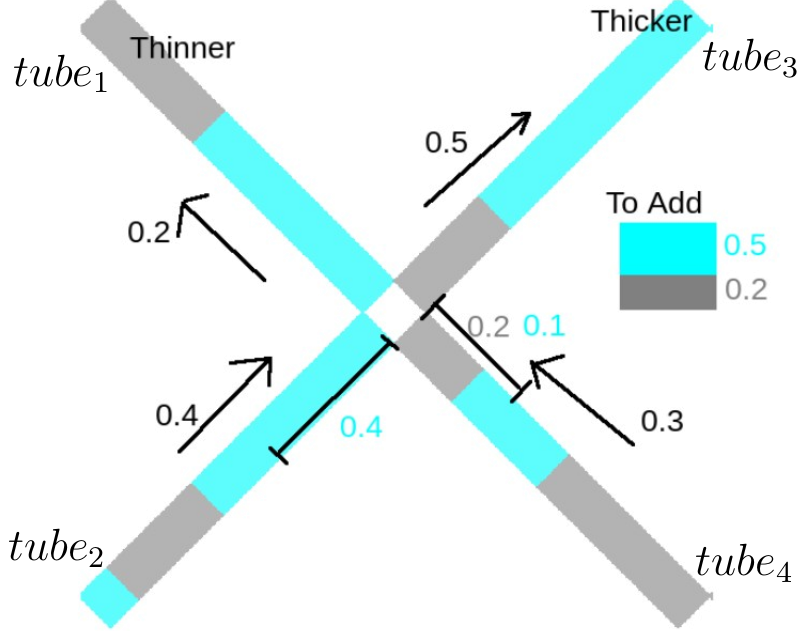
\includegraphics[height=8cm]{fig_distributing_phases_initial}
		\caption{Distribution prediction of different fluids in a node.}
		\label{fig:distributing_phases_initial}
	\end{figure}
	
	In figure \ref{fig:distributing_phases_initial}, let us denote the tubes in the following way:
		
	\begin{enumerate}
		\item top-left, ${tube}_1$
		\item top-right, ${tube}_2$
		\item bottom-left, ${tube}_3$
		\item bottom-right, ${tube}_4$
	\end{enumerate}
	
	Here, fluid flows from ${tube}_3$ and ${tube}_4$ into ${tube}_1$ and ${tube}_2$. 

	From the calculation of flow rates, we determined that $0.7 u.v.$ (unit volumes) of fluid enters the node, while $0.7 u.v.$ exits the node. They must be equal due to Kirchhoff's law at the node. The total inflow of $0.7 u.v.$ consists of $0.4 u.v.$ from ${tube}_3$ and $0.3 u.v.$ from ${tube}_4$. The outflow consists of $0.2 u.v.$ into ${tube}_1$, and $0.5 u.v.$ into ${tube}_2$.
	
	Step-1, we calculate the sum of volume of each type of fluid flowing into the node. Here, ${tube}_3$ provides $0.4 u.v.$ of cyan fluid, while ${tube}_4$ provides $0.1 u.v.$ of cyan fluid and $0.2 u.v.$ of gray fluid. Summing we obtain $0.5 u.v.$ of cyan fluid and $0.2 u.v.$ of gray fluid, which needs to be distributed to the outflow tubes.
	
	\begin{figure}[H]
		\centering
		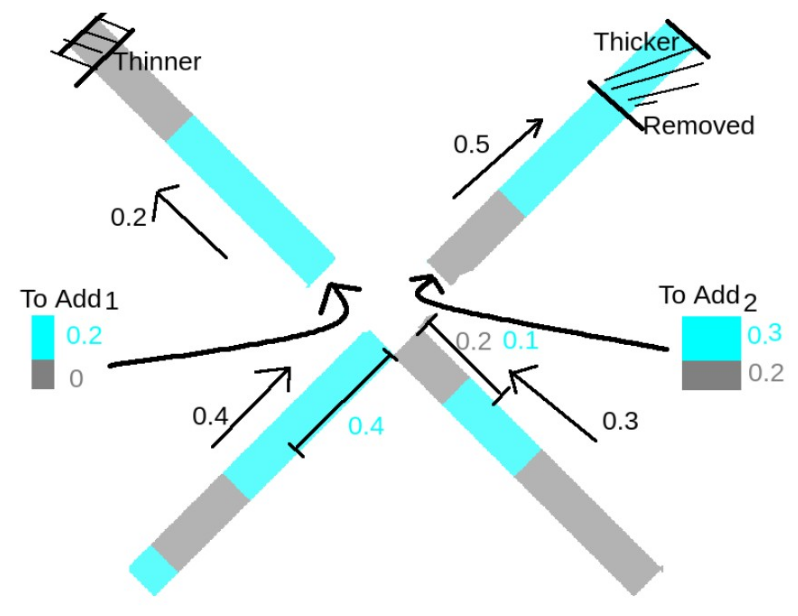
\includegraphics[height=8cm]{fig_distributing_phases_intermediary}
		\caption{Adding wetting phase to the thinner tube first.}
	\end{figure}
	
	Step-2, we allocate this $0.5 u.V.$ of cyan fluid first into the thinner tube. The thinner ${tube}_1$ takes in $0.2 u.V.$. This allocation space is entirely filled by $0.2 u.V.$ of cyan fluid. Then for the thicker tube, we need to insert $0.5 u.V.$ of fluid into it. $0.3 u.V.$ of cyan fluid is inserted first then $0.2 u.V.$ of gray fluid.
	
	\begin{figure}[H]
		\centering
		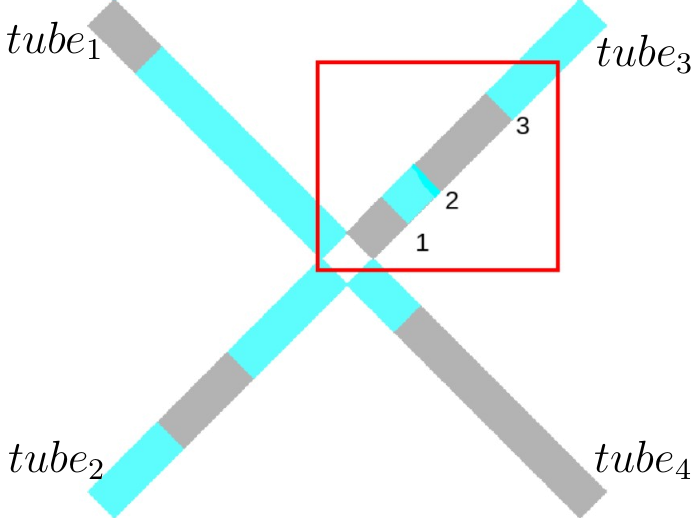
\includegraphics[height=8cm]{fig_distributing_phases_final}
		\caption{Final tube configuration with 3 menisci.}
		\label{fig:distributing_phases_final}
	\end{figure}
	
	In figure \ref{fig:distributing_phases_final}, ${tube}_1$ retains the only meniscus because the end connected to the node initially contained cyan fluid, and we introduced $0.2 u.V.$ of more cyan fluid. The single meniscus was just displaced upwards.
	
	However, in ${tube}_2$, gray fluid was on the end of the tube connected to the node. We added $0.3 u.V.$ of cyan and $0.2 u.V.$ of gray fluid. Since the cyan fluid entered the thicker tube first, we end up with 3 menisci.	

\subsection{Recombination} \label{sec:recombination-details}
	Our data structure was constrained to only allow the case for a maximum of two menisci in a tube. However, we see that in figure \ref{fig:distributing_phases_final} that there is possibility of more than 2 menisci occurring after distribution. We show the cases of distributing fluid in the nodes, which results in more than 2 menisci.
	
	\begin{figure}[H]
		\centering
		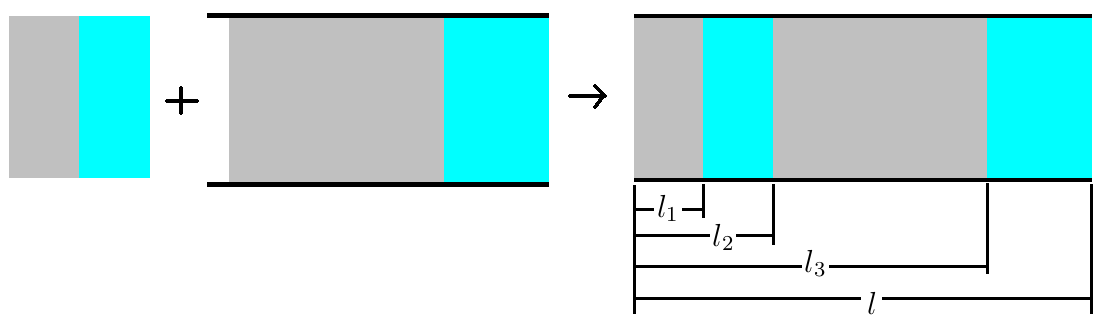
\includegraphics[width=1.0\textwidth]{fig_center-of-mass_1}
		\caption{Recombination of 3 menisci}
		\label{fig_center-of-mass_1}
	\end{figure}
	
	In figure \ref{fig_center-of-mass_1} we have a known amount of cyan and gray fluid which we need to insert into the tube. The tube which already consists of both the fluids. The flow is from left to right, so we insert the incoming fluids on the left end of the tube. Note that a block of cyan fluid always ends up in the center as it enters the tube first.
	
	Let $l_{i}$ denote the location of a meniscus. Since the tube is cylinder, the mass is simply proportional to the length they occupy in the tube, they are given by:
	
	\begin{equation}
		m_1 = l_2 - l_1 
	\end{equation}
	
	\begin{equation}
		m_2 = l - l_3
	\end{equation}
	
	Their respective center of masses $d_1$ and $d_2$ are given by:
	
	\begin{equation}	
		d_1 = \frac{l_1 + l_2}{2}
	\end{equation}
	
	\begin{equation}	
		d_2 = \frac{(l_3 + l)}{2}
	\end{equation}
	
	The center of mass of the cyan fluid in the tube is then given by:
	\begin{equation}
		d = \frac{m_1 d_1 + m_2 d_2}{m}
	\end{equation}
	
	Here,
	\begin{equation}
		m = m_1 + m_2
	\end{equation}
	
	
	We do not change the proportion of fluids in a tube during recombination. Therefore, it can be shown that if we recombine the fluids in a tube such that the center of mass of one of the fluid remained the same, then the center of mass of the other fluid will also remain the same.
	
	\begin{figure}[H]
		\centering
		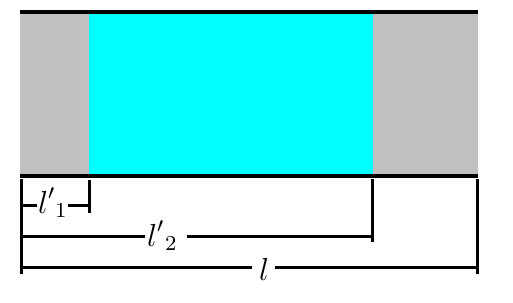
\includegraphics[width=0.5\textwidth]{fig_center-of-mass_final}
		\caption{After recombination}
	\end{figure}
	
	Let ${l'}_i$ denote the position of meniscus after recombination.
	
	\begin{equation}
		{l'}_1 = d - \frac{m}{2}
	\end{equation}
	
	\begin{equation}
		{l'}_2 = d + \frac{m}{2}
	\end{equation}
	

	\begin{figure}[H]
		\centering
		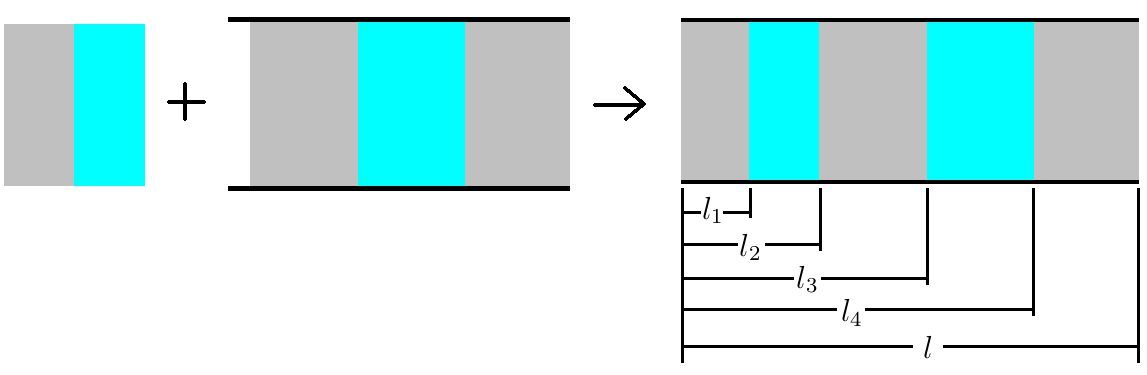
\includegraphics[width=1.0\textwidth]{fig_center-of-mass_2}
		\caption{Recombination of 4 menisci}
	\end{figure}
	
	When there are 4 menisci, we repeat the same process, except here:
	\begin{equation}
		m_2 = l_4 - l_3
	\end{equation}
	
	And
	
	\begin{equation}	
		d_2 = \frac{(l_3 + l_4)}{2}
	\end{equation}
